% Options for packages loaded elsewhere
\PassOptionsToPackage{unicode}{hyperref}
\PassOptionsToPackage{hyphens}{url}
%
\documentclass[
]{article}
\usepackage{lmodern}
\usepackage{amssymb,amsmath}
\usepackage{ifxetex,ifluatex}
\ifnum 0\ifxetex 1\fi\ifluatex 1\fi=0 % if pdftex
  \usepackage[T1]{fontenc}
  \usepackage[utf8]{inputenc}
  \usepackage{textcomp} % provide euro and other symbols
\else % if luatex or xetex
  \usepackage{unicode-math}
  \defaultfontfeatures{Scale=MatchLowercase}
  \defaultfontfeatures[\rmfamily]{Ligatures=TeX,Scale=1}
\fi
% Use upquote if available, for straight quotes in verbatim environments
\IfFileExists{upquote.sty}{\usepackage{upquote}}{}
\IfFileExists{microtype.sty}{% use microtype if available
  \usepackage[]{microtype}
  \UseMicrotypeSet[protrusion]{basicmath} % disable protrusion for tt fonts
}{}
\makeatletter
\@ifundefined{KOMAClassName}{% if non-KOMA class
  \IfFileExists{parskip.sty}{%
    \usepackage{parskip}
  }{% else
    \setlength{\parindent}{0pt}
    \setlength{\parskip}{6pt plus 2pt minus 1pt}}
}{% if KOMA class
  \KOMAoptions{parskip=half}}
\makeatother
\usepackage{xcolor}
\IfFileExists{xurl.sty}{\usepackage{xurl}}{} % add URL line breaks if available
\IfFileExists{bookmark.sty}{\usepackage{bookmark}}{\usepackage{hyperref}}
\hypersetup{
  pdftitle={Trabajo con imágenes},
  pdfauthor={Fernando Gomez Perera, Ricardo Vargas Kumul y Calvin Lopez Alvarez},
  hidelinks,
  pdfcreator={LaTeX via pandoc}}
\urlstyle{same} % disable monospaced font for URLs
\usepackage[margin=1in]{geometry}
\usepackage{color}
\usepackage{fancyvrb}
\newcommand{\VerbBar}{|}
\newcommand{\VERB}{\Verb[commandchars=\\\{\}]}
\DefineVerbatimEnvironment{Highlighting}{Verbatim}{commandchars=\\\{\}}
% Add ',fontsize=\small' for more characters per line
\usepackage{framed}
\definecolor{shadecolor}{RGB}{255,255,255}
\newenvironment{Shaded}{\begin{snugshade}}{\end{snugshade}}
\newcommand{\AlertTok}[1]{\textcolor[rgb]{0.75,0.01,0.01}{\textbf{\colorbox[rgb]{0.97,0.90,0.90}{#1}}}}
\newcommand{\AnnotationTok}[1]{\textcolor[rgb]{0.79,0.38,0.79}{#1}}
\newcommand{\AttributeTok}[1]{\textcolor[rgb]{0.00,0.34,0.68}{#1}}
\newcommand{\BaseNTok}[1]{\textcolor[rgb]{0.69,0.50,0.00}{#1}}
\newcommand{\BuiltInTok}[1]{\textcolor[rgb]{0.39,0.29,0.61}{\textbf{#1}}}
\newcommand{\CharTok}[1]{\textcolor[rgb]{0.57,0.30,0.62}{#1}}
\newcommand{\CommentTok}[1]{\textcolor[rgb]{0.54,0.53,0.53}{#1}}
\newcommand{\CommentVarTok}[1]{\textcolor[rgb]{0.00,0.58,1.00}{#1}}
\newcommand{\ConstantTok}[1]{\textcolor[rgb]{0.67,0.33,0.00}{#1}}
\newcommand{\ControlFlowTok}[1]{\textcolor[rgb]{0.12,0.11,0.11}{\textbf{#1}}}
\newcommand{\DataTypeTok}[1]{\textcolor[rgb]{0.00,0.34,0.68}{#1}}
\newcommand{\DecValTok}[1]{\textcolor[rgb]{0.69,0.50,0.00}{#1}}
\newcommand{\DocumentationTok}[1]{\textcolor[rgb]{0.38,0.47,0.50}{#1}}
\newcommand{\ErrorTok}[1]{\textcolor[rgb]{0.75,0.01,0.01}{\underline{#1}}}
\newcommand{\ExtensionTok}[1]{\textcolor[rgb]{0.00,0.58,1.00}{\textbf{#1}}}
\newcommand{\FloatTok}[1]{\textcolor[rgb]{0.69,0.50,0.00}{#1}}
\newcommand{\FunctionTok}[1]{\textcolor[rgb]{0.39,0.29,0.61}{#1}}
\newcommand{\ImportTok}[1]{\textcolor[rgb]{1.00,0.33,0.00}{#1}}
\newcommand{\InformationTok}[1]{\textcolor[rgb]{0.69,0.50,0.00}{#1}}
\newcommand{\KeywordTok}[1]{\textcolor[rgb]{0.12,0.11,0.11}{\textbf{#1}}}
\newcommand{\NormalTok}[1]{\textcolor[rgb]{0.12,0.11,0.11}{#1}}
\newcommand{\OperatorTok}[1]{\textcolor[rgb]{0.12,0.11,0.11}{#1}}
\newcommand{\OtherTok}[1]{\textcolor[rgb]{0.00,0.43,0.16}{#1}}
\newcommand{\PreprocessorTok}[1]{\textcolor[rgb]{0.00,0.43,0.16}{#1}}
\newcommand{\RegionMarkerTok}[1]{\textcolor[rgb]{0.00,0.34,0.68}{\colorbox[rgb]{0.88,0.91,0.97}{#1}}}
\newcommand{\SpecialCharTok}[1]{\textcolor[rgb]{0.24,0.68,0.91}{#1}}
\newcommand{\SpecialStringTok}[1]{\textcolor[rgb]{1.00,0.33,0.00}{#1}}
\newcommand{\StringTok}[1]{\textcolor[rgb]{0.75,0.01,0.01}{#1}}
\newcommand{\VariableTok}[1]{\textcolor[rgb]{0.00,0.34,0.68}{#1}}
\newcommand{\VerbatimStringTok}[1]{\textcolor[rgb]{0.75,0.01,0.01}{#1}}
\newcommand{\WarningTok}[1]{\textcolor[rgb]{0.75,0.01,0.01}{#1}}
\usepackage{graphicx}
\makeatletter
\def\maxwidth{\ifdim\Gin@nat@width>\linewidth\linewidth\else\Gin@nat@width\fi}
\def\maxheight{\ifdim\Gin@nat@height>\textheight\textheight\else\Gin@nat@height\fi}
\makeatother
% Scale images if necessary, so that they will not overflow the page
% margins by default, and it is still possible to overwrite the defaults
% using explicit options in \includegraphics[width, height, ...]{}
\setkeys{Gin}{width=\maxwidth,height=\maxheight,keepaspectratio}
% Set default figure placement to htbp
\makeatletter
\def\fps@figure{htbp}
\makeatother
\setlength{\emergencystretch}{3em} % prevent overfull lines
\providecommand{\tightlist}{%
  \setlength{\itemsep}{0pt}\setlength{\parskip}{0pt}}
\setcounter{secnumdepth}{-\maxdimen} % remove section numbering
\ifluatex
  \usepackage{selnolig}  % disable illegal ligatures
\fi

\title{Trabajo con imágenes}
\author{Fernando Gomez Perera, Ricardo Vargas Kumul y Calvin Lopez
Alvarez}
\date{r Sys.Date()}

\begin{document}
\maketitle

\begin{center}\rule{0.5\linewidth}{0.5pt}\end{center}

\hypertarget{aplicaciuxf3n}{%
\section{Aplicación}\label{aplicaciuxf3n}}

El objetivo es crear una aplicación donde se muestre como salida la
información detallada de cada mamografía.

\hypertarget{extracciuxf3n-y-limpieza-de-imagenes}{%
\subsection{Extracción y Limpieza de
Imagenes}\label{extracciuxf3n-y-limpieza-de-imagenes}}

Extraemos la informacion detallada de cada mamografía del archivo
info.txt, posteriormente realizar correccione sobre este para permitir
su uso dentro de la app. Al terminar lo almacenamos en un .csv para
usarlo más adelante en el proyecto.

\begin{Shaded}
\begin{Highlighting}[]
\CommentTok{\# Extraer la información detallada de cada mamografía}
\NormalTok{pacman}\SpecialCharTok{::}\FunctionTok{p\_load}\NormalTok{(fs, readr, dplyr, furrr, purrr, forcats, stringr, pixmap, png)}

\CommentTok{\# Leer el archivo info.txt con la información detallada de cada mamografía}
\NormalTok{info }\OtherTok{\textless{}{-}} \FunctionTok{path}\NormalTok{(}\StringTok{"extdata/all{-}mias/Info.txt"}\NormalTok{) }\SpecialCharTok{\%\textgreater{}\%}
  \CommentTok{\# Llevar a cabo algunas correcciones para obtener de forma correcta la información dentro del archivo}
  \FunctionTok{read\_delim}\NormalTok{(}\AttributeTok{delim =} \StringTok{" "}\NormalTok{,}
             \AttributeTok{col\_names =} \FunctionTok{c}\NormalTok{(}\StringTok{"ref"}\NormalTok{, }\StringTok{"bg\_tissue"}\NormalTok{, }\StringTok{"abnorm"}\NormalTok{, }\StringTok{"severity"}\NormalTok{, }\StringTok{"x"}\NormalTok{, }\StringTok{"y"}\NormalTok{, }\StringTok{"approx\_radius"}\NormalTok{),}
             \AttributeTok{col\_types =} \StringTok{"cccciii"}\NormalTok{,}
             \AttributeTok{skip =} \DecValTok{102}\NormalTok{, }\AttributeTok{n\_max =} \DecValTok{330}\NormalTok{)}

\CommentTok{\# Almacenar el resultado en un CSV sin pre{-}procesar para poder usarlo en las otras fases del proyecto}
\FunctionTok{write\_csv}\NormalTok{(info, }\AttributeTok{file =} \FunctionTok{path}\NormalTok{(}\StringTok{"extdata/all{-}mias/info.csv"}\NormalTok{))}
\end{Highlighting}
\end{Shaded}

\hypertarget{pre-precesamiento-de-datos}{%
\subsection{Pre-precesamiento de
datos}\label{pre-precesamiento-de-datos}}

Los caracteres son convertidos en factores para ser re-codificados y nos
permitan mostrarlos adecuadamente en la app.

\begin{Shaded}
\begin{Highlighting}[]
\CommentTok{\# Pre{-}procesar el resultado para poder usarlo dentro de la app de Shiny}
\NormalTok{info }\OtherTok{\textless{}{-}}\NormalTok{ info }\SpecialCharTok{\%\textgreater{}\%}
  \CommentTok{\# Convertir los caracteres en factores}
  \FunctionTok{mutate}\NormalTok{(}\FunctionTok{across}\NormalTok{(}\FunctionTok{where}\NormalTok{(is.character), as.factor)) }\SpecialCharTok{\%\textgreater{}\%}
  \CommentTok{\# Re{-}codificar los factores}
  \FunctionTok{mutate}\NormalTok{(}
    \AttributeTok{bg\_tissue =} \FunctionTok{fct\_recode}\NormalTok{(}
\NormalTok{      bg\_tissue,}
      \StringTok{"Graso"} \OtherTok{=} \StringTok{"F"}\NormalTok{,}
      \StringTok{"Graso{-}glandular"} \OtherTok{=} \StringTok{"G"}\NormalTok{,}
      \StringTok{"Glandular{-}denso"} \OtherTok{=} \StringTok{"D"}
\NormalTok{    ),}
    \AttributeTok{abnorm =} \FunctionTok{fct\_recode}\NormalTok{(}
\NormalTok{      abnorm,}
      \StringTok{"Calcificación"} \OtherTok{=} \StringTok{"CALC"}\NormalTok{,}
      \StringTok{"Masas bien definidas o circunscritas"} \OtherTok{=} \StringTok{"CIRC"}\NormalTok{,}
      \StringTok{"Masa espigada"} \OtherTok{=} \StringTok{"SPIC"}\NormalTok{,}
      \StringTok{"Otras masas o mal definidas"} \OtherTok{=} \StringTok{"MISC"}\NormalTok{,}
      \StringTok{"Distorsión estructural"} \OtherTok{=} \StringTok{"ARCH"}\NormalTok{,}
      \StringTok{"Asimetría"} \OtherTok{=} \StringTok{"ASYM"}\NormalTok{,}
      \StringTok{"Normal"} \OtherTok{=} \StringTok{"NORM"}
\NormalTok{    ),}
    \AttributeTok{severity =} \FunctionTok{fct\_recode}\NormalTok{(}
\NormalTok{      severity,}
      \StringTok{"Benigno"} \OtherTok{=} \StringTok{"B"}\NormalTok{,}
      \StringTok{"Maligno"} \OtherTok{=} \StringTok{"M"}
\NormalTok{    )}
\NormalTok{  )}

\CommentTok{\# Almacenar el resultado en un archivo RData para su uso dentro de la aplicación}
\FunctionTok{save}\NormalTok{(info, }\AttributeTok{file =} \FunctionTok{path}\NormalTok{(}\StringTok{"app/info.RData"}\NormalTok{))}
\end{Highlighting}
\end{Shaded}

\hypertarget{conversiuxf3n-de-pgm-a-png}{%
\subsection{Conversión de PGM a PNG}\label{conversiuxf3n-de-pgm-a-png}}

Finalmente realizamos la convesión de las imagenes de su formato
original (PGM) a uno que pueda ser visualizado dentro de nuestra app
(PNG).

\begin{Shaded}
\begin{Highlighting}[]
\CommentTok{\# Función para convertir las imágenes en formato PGM a formato PNG para poder visualizarlas dentro de la aplicación}
\NormalTok{pnm\_to\_png }\OtherTok{\textless{}{-}} \ControlFlowTok{function}\NormalTok{(filename, new\_filename) \{}
  \CommentTok{\# Leer la imagen en formato PGM}
\NormalTok{  img }\OtherTok{\textless{}{-}} \FunctionTok{read.pnm}\NormalTok{(filename)}
  \CommentTok{\# Almacenar la imagen en formato PNG manteniendo sus dimensiones originales}
  \FunctionTok{png}\NormalTok{(new\_filename, }\AttributeTok{width =}\NormalTok{ img}\SpecialCharTok{@}\NormalTok{size[}\DecValTok{1}\NormalTok{], }\AttributeTok{height =}\NormalTok{ img}\SpecialCharTok{@}\NormalTok{size[}\DecValTok{2}\NormalTok{])}
  \FunctionTok{plot}\NormalTok{(img)}
  \FunctionTok{dev.off}\NormalTok{()}
\NormalTok{\}}

\CommentTok{\# Crear un nuevo directorio para almacenar las imágenes en formato PNG dentro del directorio de la aplicación}
\FunctionTok{dir\_create}\NormalTok{(}\StringTok{"app/img"}\NormalTok{)}

\CommentTok{\# Obtener la ubicación de cada imagen en formato PGM}
\NormalTok{img\_paths }\OtherTok{\textless{}{-}} \FunctionTok{dir\_ls}\NormalTok{(}\StringTok{"extdata/all{-}mias/"}\NormalTok{, }\AttributeTok{glob =} \StringTok{"*.pgm"}\NormalTok{)}

\CommentTok{\# Crear una nueva ubicación para cada imagen en formato PNG}
\NormalTok{new\_img\_paths }\OtherTok{\textless{}{-}} \FunctionTok{path}\NormalTok{(}\StringTok{"app/img"}\NormalTok{, }\FunctionTok{str\_extract}\NormalTok{(img\_paths, }\AttributeTok{pattern =} \StringTok{"(?\textless{}=mdb0\{0,2\})[1{-}9]\{1\}[:digit:]\{0,2\}"}\NormalTok{), }\AttributeTok{ext =} \StringTok{"png"}\NormalTok{)}

\CommentTok{\# Paralelizar la conversión de las imágenes para que el proceso termine más rápido}
\FunctionTok{plan}\NormalTok{(multisession, }\AttributeTok{workers =} \DecValTok{4}\NormalTok{)}

\CommentTok{\# Convertir las imágenes en formato PGM a formato PNG}
\FunctionTok{future\_map2}\NormalTok{(img\_paths, new\_img\_paths, }\SpecialCharTok{\textasciitilde{}} \FunctionTok{pnm\_to\_png}\NormalTok{(.x, .y))}
\end{Highlighting}
\end{Shaded}

\hypertarget{demostraciuxf3n-de-la-aplicaciuxf3n}{%
\subsection{Demostración de la
Aplicación}\label{demostraciuxf3n-de-la-aplicaciuxf3n}}

La aplicación se encuentra divdida en 2 partes.

\hypertarget{informaciuxf3n-de-todas-las-mamografuxedas}{%
\subsubsection{Información de todas las
mamografías}\label{informaciuxf3n-de-todas-las-mamografuxedas}}

Muestra la información importante de cada imagen como son tejido,
anormalidad, diagnóstico y coordenadas de la anormalidad. Se agregaron
filtros para facilitar la busqueda de casos específicos.

\begin{figure}
\centering
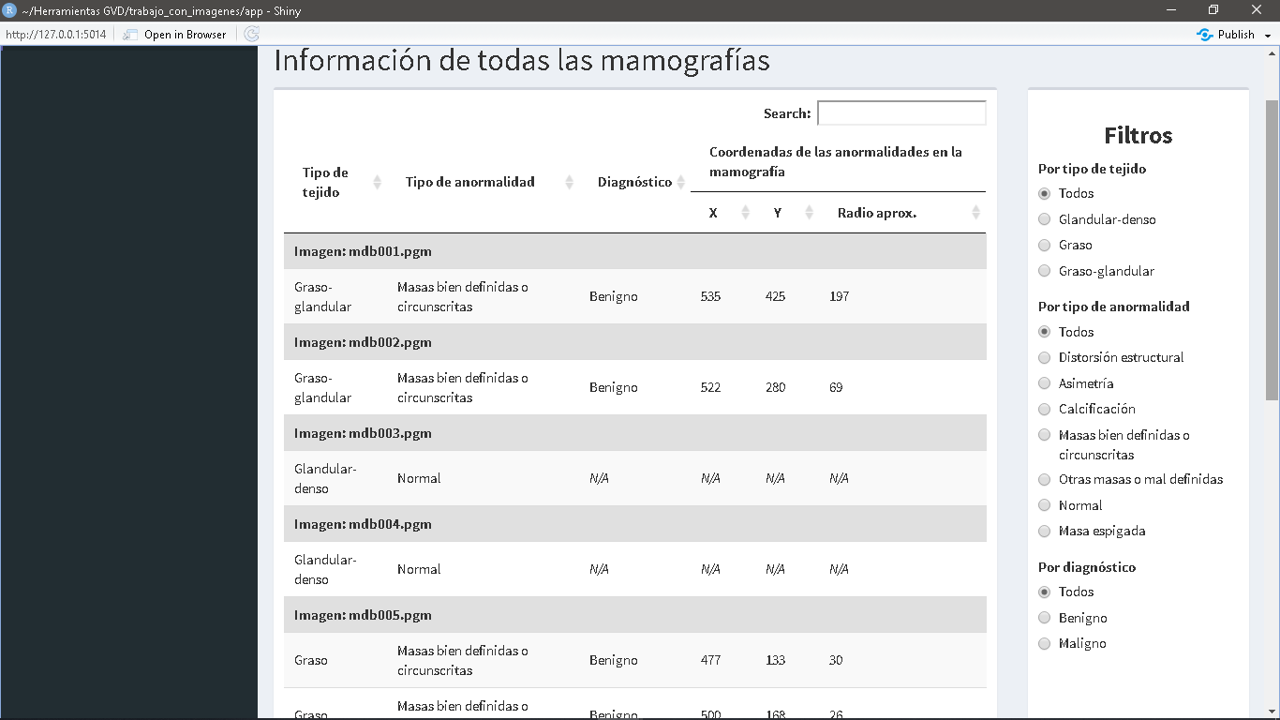
\includegraphics{img/app_1.png}
\caption{RE}
\end{figure}

\hypertarget{informaciuxf3n-por-mamografuxeda}{%
\subsubsection{Información por
mamografía}\label{informaciuxf3n-por-mamografuxeda}}

Presenta la información disponible de una manera detallada sobre cada
imagen de manera individual, contiene la misma informacion que la
sección anterior pero sumando la representación visual de la mamografía
la cual ayuda a identificar los detalles dentro de la misma

\begin{figure}
\centering
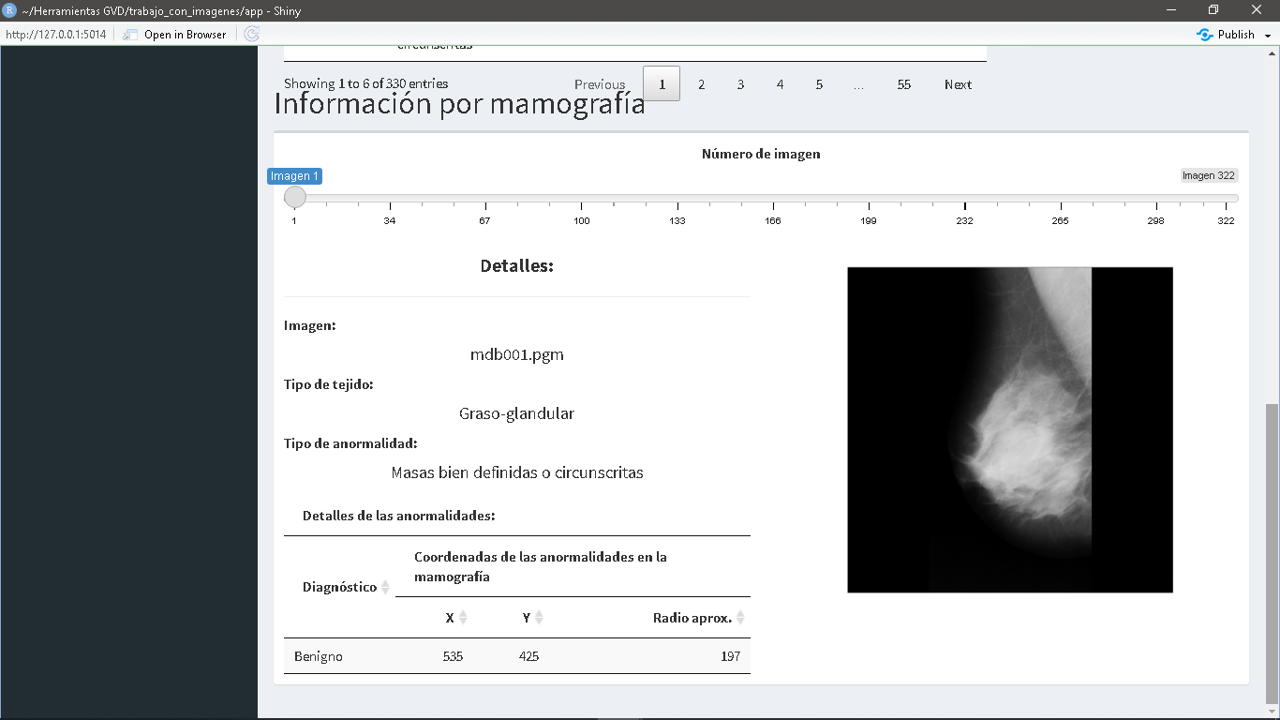
\includegraphics{img/app_2.png}
\caption{RE}
\end{figure}

\hypertarget{limpieza-de-imagen}{%
\section{Limpieza de Imagen}\label{limpieza-de-imagen}}

El objetivo es replicar un proceso de limpieza del fondo de la imagen

\begin{Shaded}
\begin{Highlighting}[]
\CommentTok{\# Bibliotecas a usar}
\ImportTok{import}\NormalTok{ os}
\ImportTok{import}\NormalTok{ re}
\ImportTok{import}\NormalTok{ cv2 }\ImportTok{as}\NormalTok{ cv}
\ImportTok{import}\NormalTok{ numpy }\ImportTok{as}\NormalTok{ np}
\ImportTok{import}\NormalTok{ matplotlib.pyplot }\ImportTok{as}\NormalTok{ plt}
\end{Highlighting}
\end{Shaded}

\hypertarget{artuxedculos-a-replicar}{%
\subsection{Artículos a replicar}\label{artuxedculos-a-replicar}}

Los artículos que usamos como referencia para desarrollar los proyectos
son los siguientes:

\begin{itemize}
\item
  \textbf{\emph{An improved GVF snake based breast region extrapolation
  scheme for digital mammograms}} de \emph{Liu et al}.: El objetivo de
  este artículo es extrapolar la región del busto usando un esquema
  mejorado de una serpiente Flujo del Vector Gradiente o \emph{Gradient
  Vector Flow (GVF) snake}.
\item
  \textbf{\emph{A pectoral muscle segmentation algorithm for digital
  mammograms using Otsu thresholding and multiple regression analysis}}
  de \emph{Liu et al}: El objetivo de este artículo es segmentar la
  región del músculo pectoral de la región del pecho combinando el
  esquema de umbralización de Otsu y el procesamiento matemático
  morfológico para obtener un borde del músculo pectoral, y usar el
  análsis de regresión múltiple (\emph{MRA}) para obtener una
  segmentación precisa del mismo.
\end{itemize}

\hypertarget{primera-parte-extrapolaciuxf3n-de-la-regiuxf3n-del-busto}{%
\subsection{Primera parte: Extrapolación de la región del
busto}\label{primera-parte-extrapolaciuxf3n-de-la-regiuxf3n-del-busto}}

Para llevarl a cabo, tomamos como referencia el primer artículo de
\emph{Liu et al}. \protect\hyperlink{ref}{{[}1{]}} En este artículo, los
autores proponen un esquema mejorado de una serpiente Flujo del Vector
Gradiente o \emph{Gradient Vector Flow (GVF) snake} para poder
extrapolar toda la región del busto. Este esquema o algoritmo que ellos
proponen es el siguiente:

\begin{figure}
\centering
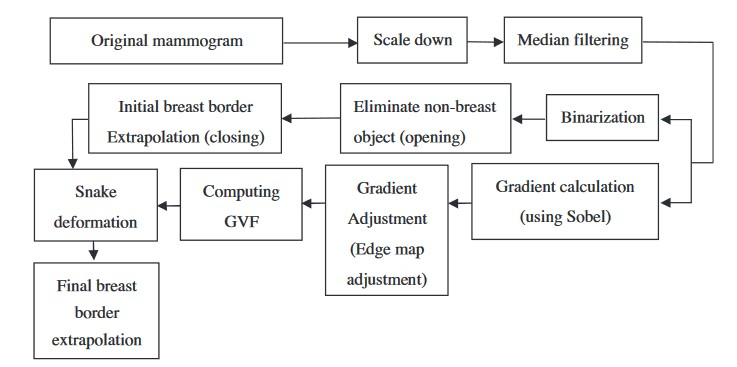
\includegraphics{img/gvf_scheme.jpg}
\caption{RE}
\end{figure}

\begin{enumerate}
\def\labelenumi{\arabic{enumi}.}
\tightlist
\item
  Reescalar las imágenes originales de las mamografías.
\item
  Aplicar un filtro de mediana a las imágenes reescaladas.
\end{enumerate}

En este punto, el proceso se divide en 2 fase:

\begin{enumerate}
\def\labelenumi{\arabic{enumi}.}
\setcounter{enumi}{2}
\tightlist
\item
  Binarizar la imagen reescalada.
\item
  Eliminar los objetos que no son de la región del busto.
\item
  Obtener une extrapolación inicial del borde del busto.
\end{enumerate}

Paralelamente:

\begin{enumerate}
\def\labelenumi{\arabic{enumi}.}
\setcounter{enumi}{2}
\tightlist
\item
  Aplicar un filtro de Sobel para obtener el campo gradiente de la
  mamografía reescalada.
\item
  Ajustar el campo gradiente.
\item
  Calcular el Flujo del Vector Gradiente (\emph{GVF}).
\end{enumerate}

En este punto, ambos procesos se unen:

\begin{enumerate}
\def\labelenumi{\arabic{enumi}.}
\setcounter{enumi}{5}
\tightlist
\item
  Aplicar la deformación serpiente usando el \emph{GVF} calculado sobre
  la extrapolación inicial del borde del busto.
\item
  Obtener la extrapolación final del borde del busto.
\end{enumerate}

\hypertarget{tarea-1}{%
\subsubsection{Tarea 1}\label{tarea-1}}

\hypertarget{replica-un-proceso-de-limpieza-del-fondo-de-la-imagen}{%
\paragraph{2. Replica un proceso de limpieza del fondo de la
imagen}\label{replica-un-proceso-de-limpieza-del-fondo-de-la-imagen}}

Este proceso sigue la primera ramificación del algoritmo propuesto por
los autores.

Primero, se importan al entorno todas las imágenes originales.

\begin{Shaded}
\begin{Highlighting}[]
\CommentTok{\# Ruta de las imágenes originales}
\NormalTok{base\_dir }\OperatorTok{=} \StringTok{\textquotesingle{}../extdata/all{-}mias/\textquotesingle{}}
\NormalTok{all\_filenames }\OperatorTok{=}\NormalTok{ os.listdir(base\_dir)}
\NormalTok{imgs\_filenames }\OperatorTok{=} \BuiltInTok{list}\NormalTok{()}

\CommentTok{\# Extraer los archivos que corresponden a las imágenes de las mamografías}
\ControlFlowTok{for}\NormalTok{ filename }\KeywordTok{in}\NormalTok{ all\_filenames:}
    \ControlFlowTok{if}\NormalTok{ filename.endswith(}\StringTok{\textquotesingle{}.pgm\textquotesingle{}}\NormalTok{):}
\NormalTok{        imgs\_filenames.append(filename)}

\CommentTok{\# Lectura de las imágenes con el parámetro {-}1 para leer la imagen sin modificar}
\NormalTok{imgs\_orig }\OperatorTok{=} \BuiltInTok{list}\NormalTok{(}\BuiltInTok{map}\NormalTok{(}\KeywordTok{lambda}\NormalTok{ img\_name: cv.imread(base\_dir}\OperatorTok{+}\NormalTok{img\_name, }\OperatorTok{{-}}\DecValTok{1}\NormalTok{), imgs\_filenames))}

\CommentTok{\# Imagen de ejemplo}
\NormalTok{plt.imshow(imgs\_orig[}\DecValTok{13}\NormalTok{], cmap}\OperatorTok{=}\StringTok{\textquotesingle{}gray\textquotesingle{}}\NormalTok{)}
\NormalTok{plt.show()}
\end{Highlighting}
\end{Shaded}

\begin{figure}
\centering
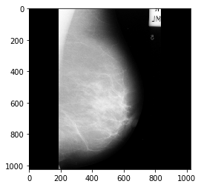
\includegraphics{img/tarea_2_0.png}
\caption{RE}
\end{figure}

\hypertarget{reescalar-la-imagen}{%
\subparagraph{2.1 Reescalar la imagen}\label{reescalar-la-imagen}}

Siguiendo el diagrama de flujo propuesto, el primer paso es reescalar la
imagen para hacerla más pequeña. Esto permitirá ahorrar tiempo en la
ejecución de los pasos.

Para mantener la calidad de la extrapolación, los autores sugieren
reescalar las imágenes originales de 1024 x 1024 pixeles a 256 x 256
pixeles.

\begin{Shaded}
\begin{Highlighting}[]
\CommentTok{\# Reescalar las imágenes para hacerlas más pequeñas (scale down)}
\NormalTok{imgs\_scale }\OperatorTok{=} \BuiltInTok{list}\NormalTok{(}\BuiltInTok{map}\NormalTok{(}\KeywordTok{lambda}\NormalTok{ img\_orig: cv.resize(img\_orig, (}\DecValTok{256}\NormalTok{, }\DecValTok{256}\NormalTok{)), imgs\_orig))}

\CommentTok{\# Imagen de ejemplo}
\NormalTok{plt.imshow(imgs\_scale[}\DecValTok{13}\NormalTok{], cmap}\OperatorTok{=}\StringTok{\textquotesingle{}gray\textquotesingle{}}\NormalTok{)}
\NormalTok{plt.show()}
\end{Highlighting}
\end{Shaded}

\begin{figure}
\centering
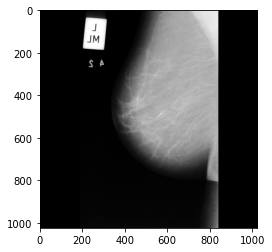
\includegraphics{img/tarea_2_1.png}
\caption{RE}
\end{figure}

\hypertarget{aplicar-el-filtro-de-mediana}{%
\subparagraph{2.2 Aplicar el filtro de
mediana}\label{aplicar-el-filtro-de-mediana}}

Los autores sugieren aplicar un filtro de mediana de 3 x 3 pixeles para
reducir el ruido de la imagen.

\begin{Shaded}
\begin{Highlighting}[]
\CommentTok{\# Aplicar un filtro de mediana a cada una de las imágenes}
\NormalTok{imgs\_filter }\OperatorTok{=} \BuiltInTok{list}\NormalTok{(}\BuiltInTok{map}\NormalTok{(}\KeywordTok{lambda}\NormalTok{ img\_scale: cv.medianBlur(img\_scale, }\DecValTok{3}\NormalTok{), imgs\_scale))}

\CommentTok{\# Imagen de ejemplo}
\NormalTok{plt.imshow(imgs\_filter[}\DecValTok{13}\NormalTok{], cmap}\OperatorTok{=}\StringTok{\textquotesingle{}gray\textquotesingle{}}\NormalTok{)}
\NormalTok{plt.show()}
\end{Highlighting}
\end{Shaded}

\begin{figure}
\centering
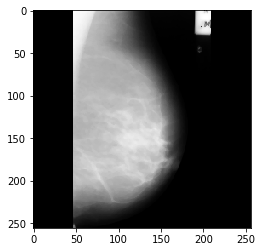
\includegraphics{img/tarea_2_2.png}
\caption{RE}
\end{figure}

\hypertarget{binarizaciuxf3n-de-las-imuxe1genes}{%
\subparagraph{2.3 Binarización de las
imágenes}\label{binarizaciuxf3n-de-las-imuxe1genes}}

Este paso permite obtener un contorno aproximado. Para ello, los autores
proponen obtener un umbrarl \(T\), el cual será equivalente al valor
medio de gris de la imagen.

La fórmula para calcular el umbral \(T\) es la siguiente:

\[T = 0.2 \cdot  \frac{\sum_{n = 0}^{255} n \cdot H(n)}{\sum_{n = 0}^{255} H(n)}\]

donde \(n\) es el valor del nivel de gris, el cual va de 0 a 255, y
\(H(n)\) es el número de pixeles con el valor de pixel \(n\) dentro de
la imagen, el cual se obtiene de su histograma.

Para binarizarla, se sigue la siguiente fórmula:

\[
IB(x, y)  = \begin{cases}
    1,\text{ si } I(x,y) \geq T,\\
    0, \text{ de otra forma}.
  \end{cases}
\]

donde \(I(x, y)\) es el valor de intensidad de cada pixel en la imagen.

De esta forma, la imagen quedará divida en la región de fondo (con valor
de pixel 0) y la región de objetos (con valor de pixel 1).

\begin{Shaded}
\begin{Highlighting}[]
\CommentTok{\# Obtener del umbral a partir del valor del nivel de gris en la imagen}
\KeywordTok{def}\NormalTok{ T(img):}
\NormalTok{    H\_n }\OperatorTok{=}\NormalTok{ np.histogram(img, bins}\OperatorTok{=}\DecValTok{256}\NormalTok{, }\BuiltInTok{range}\OperatorTok{=}\NormalTok{(}\DecValTok{0}\NormalTok{, }\DecValTok{256}\NormalTok{))[}\DecValTok{0}\NormalTok{]}
    \ControlFlowTok{return} \FloatTok{0.2} \OperatorTok{*}\NormalTok{ np.}\BuiltInTok{sum}\NormalTok{(np.arange(}\DecValTok{0}\NormalTok{, }\DecValTok{256}\NormalTok{) }\OperatorTok{*}\NormalTok{ H\_n) }\OperatorTok{/}\NormalTok{ np.}\BuiltInTok{sum}\NormalTok{(H\_n)}

\CommentTok{\# Binarizar la imagen}
\KeywordTok{def}\NormalTok{ binarization(img):}
    \ControlFlowTok{return}\NormalTok{ np.where(img }\OperatorTok{\textgreater{}=}\NormalTok{ T(img), }\DecValTok{1}\NormalTok{, }\DecValTok{0}\NormalTok{).astype(np.uint8)}

\CommentTok{\# Binarización de las imágenes}
\NormalTok{imgs\_bin }\OperatorTok{=} \BuiltInTok{list}\NormalTok{(}\BuiltInTok{map}\NormalTok{(}\KeywordTok{lambda}\NormalTok{ img\_filter: binarization(img\_filter), imgs\_filter))}

\CommentTok{\# Imagen de ejemplo}
\NormalTok{plt.imshow(imgs\_bin[}\DecValTok{13}\NormalTok{], cmap}\OperatorTok{=}\StringTok{\textquotesingle{}gray\textquotesingle{}}\NormalTok{)}
\NormalTok{plt.show()}
\end{Highlighting}
\end{Shaded}

\begin{figure}
\centering
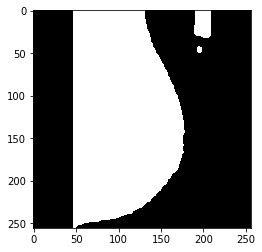
\includegraphics{img/tarea_2_3.png}
\caption{RE}
\end{figure}

\hypertarget{eliminar-los-objetos-que-no-son-parte-de-la-regiuxf3n-del-busto.}{%
\subparagraph{2.4 Eliminar los objetos que no son parte de la región del
busto.}\label{eliminar-los-objetos-que-no-son-parte-de-la-regiuxf3n-del-busto.}}

Este proceso está compuesto de 2 partes:

2.4.1 Procesamiento morfológico

Tomando como base el ejemplo de la imagen binarizada, se puede notar que
además de la región del busto, hay pequeñas regiones que no son de
interés. Para eliminarlos, los autores proponen en su algoritmo aplicar
la operación morfológica de apertura, la cual está compuesta de 2
transformaciones morfológicas:

\begin{itemize}
\tightlist
\item
  La \textbf{erosión}, la cual, como dice su nombre, erosiona los
  límites del objeto en primer plano (siempre trata de mantener el
  primer plano en blanco).
\item
  La \textbf{dilatación}, que es lo opuesto a la erosión. Esto provoca
  que aumente la región blanca en la imagen o aumente el tamaño del
  objeto en primer plano.
\end{itemize}

Para ello, la función toma un kernel que se desliza por la imagen, y
modfica el valor de un pixel de acuerdo con los siguientes criterios:

\begin{itemize}
\tightlist
\item
  En el caso de la \textbf{erosión}, el valor del pixel será de 1
  solamente si todos los pixeles bajo el kernel son 1. Sino, se erosiona
  (se vuelve 0).
\item
  En el caso de la \textbf{dilatación}, el valor del pixel será de 1 si
  al menos un pixel bajo el kernel es de 1.
\end{itemize}

Los autores proponen usar un elemento estructurado (kernel) formado por
un disco de radio 2 pixeles.

\begin{Shaded}
\begin{Highlighting}[]
\CommentTok{\# Creación del kernel compuesto por un disco de radio 2}
\NormalTok{kernel }\OperatorTok{=}\NormalTok{ cv.getStructuringElement(cv.MORPH\_ELLIPSE, (}\DecValTok{5}\NormalTok{, }\DecValTok{5}\NormalTok{))}
\NormalTok{kernel}
\end{Highlighting}
\end{Shaded}

array({[}{[}0, 0, 1, 0, 0{]},\\
\hspace*{0.333em}\hspace*{0.333em}\hspace*{0.333em}\hspace*{0.333em}\hspace*{0.333em}\hspace*{0.333em}\hspace*{0.333em}{[}1,
1, 1, 1, 1{]},\\
\hspace*{0.333em}\hspace*{0.333em}\hspace*{0.333em}\hspace*{0.333em}\hspace*{0.333em}\hspace*{0.333em}\hspace*{0.333em}{[}1,
1, 1, 1, 1{]},\\
\hspace*{0.333em}\hspace*{0.333em}\hspace*{0.333em}\hspace*{0.333em}\hspace*{0.333em}\hspace*{0.333em}\hspace*{0.333em}{[}1,
1, 1, 1, 1{]},\\
\hspace*{0.333em}\hspace*{0.333em}\hspace*{0.333em}\hspace*{0.333em}\hspace*{0.333em}\hspace*{0.333em}\hspace*{0.333em}{[}0,
0, 1, 0, 0{]}{]}, dtype=uint8)

\begin{Shaded}
\begin{Highlighting}[]
\CommentTok{\# Aplicar el procesamiento morfológico de apertura sobre las imágenes binarizadas}
\NormalTok{imgs\_mpo }\OperatorTok{=} \BuiltInTok{list}\NormalTok{(}\BuiltInTok{map}\NormalTok{(}\KeywordTok{lambda}\NormalTok{ img\_bin: cv.morphologyEx(img\_bin, cv.MORPH\_OPEN, kernel), imgs\_bin))}

\CommentTok{\# Imagen de ejemplo}
\NormalTok{plt.imshow(imgs\_mpo[}\DecValTok{13}\NormalTok{], cmap}\OperatorTok{=}\StringTok{\textquotesingle{}gray\textquotesingle{}}\NormalTok{)}
\NormalTok{plt.show()}
\end{Highlighting}
\end{Shaded}

\begin{figure}
\centering
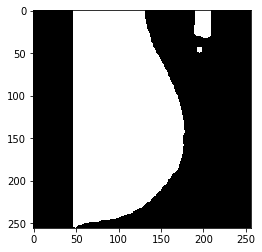
\includegraphics{img/tarea_2_4.png}
\caption{RE}
\end{figure}

Aún después de aplicar esta operación, y como se visualiza en la imagen
de ejemplo, aún quedan elementos que no corresponden al área del busto.
Sin embargo, claramente se puede notar que su tamaño es menor en
comparación al área del busto.

Por ello, para eliminar los elementos faltantes, los autores proponen
usar las características del objeto busto en la imagen mamográfica para
etiquetar los objetos, y después extraer el objeto de mayor tamaño de la
imagen binarizada. Y aquellos objetos que no correspondan al área del
busto se modifican para volverse parte del fondo en dicha imagen.
Finalmente, estos objetos también se modifican en la imagen reducida
\(I\), estableciendo sus valores de intensidad igual al nivel de gris
medio del área que no pertenece al área del busto en \(I\).

Sin embargo, los autores no explican cómo llevaron a cabo este proceso.
Por lo que nosotros implementamos un proceso que busca replicar los
puntos que ellos mencionan.

Este proceso se compone de los siguientes pasos, aplicados a cada
mamografía:

\begin{enumerate}
\def\labelenumi{\arabic{enumi}.}
\tightlist
\item
  Obtener los contornos de los objetos en la imagen binarizada ya
  modificada por el procesamiento morfológico de apertura.
\item
  Tomar el contorno del objeto más grande, que corresponde a la región
  del busto.
\item
  Crear una nueva imagen binarizada pintando solamente la región del
  objeto más grande.
\item
  Limpiar la mamografía, estableciendo las intensidades de los objetos
  que no son parte de la región del busto con el valor del nivel de gris
  medio del área que no pertenece al busto.
\end{enumerate}

\begin{Shaded}
\begin{Highlighting}[]
\CommentTok{\# Obtener el contorno del objeto más grande en la imagen binarizada procesada}
\KeywordTok{def}\NormalTok{ get\_max\_contour(img\_mpo):}
\NormalTok{    \_, contours, \_ }\OperatorTok{=}\NormalTok{ cv.findContours(img\_mpo, cv.RETR\_EXTERNAL, cv.CHAIN\_APPROX\_SIMPLE)}
    \CommentTok{\# Se obtiene el contorno del objeto más grande}
    \ControlFlowTok{return}\NormalTok{ [}\BuiltInTok{max}\NormalTok{(}\BuiltInTok{enumerate}\NormalTok{(contours), key }\OperatorTok{=} \KeywordTok{lambda}\NormalTok{ tup: }\BuiltInTok{len}\NormalTok{(tup[}\DecValTok{1}\NormalTok{]))[}\DecValTok{1}\NormalTok{]]}

\CommentTok{"""Obtener los objetos que no son la región del busto en la}
\CommentTok{imagen binarizada original"""}
\KeywordTok{def}\NormalTok{ get\_non\_breast\_objs(img\_bin):}
\NormalTok{    \_, contours, \_ }\OperatorTok{=}\NormalTok{ cv.findContours(img\_bin, cv.RETR\_EXTERNAL, cv.CHAIN\_APPROX\_SIMPLE)}
    \CommentTok{\# Se obtiene el índice del contorno del objeto más grande}
\NormalTok{    ind\_max\_contour }\OperatorTok{=} \BuiltInTok{max}\NormalTok{(}\BuiltInTok{enumerate}\NormalTok{(contours), key }\OperatorTok{=} \KeywordTok{lambda}\NormalTok{ tup: }\BuiltInTok{len}\NormalTok{(tup[}\DecValTok{1}\NormalTok{]))[}\DecValTok{0}\NormalTok{]}
    \CommentTok{\# Se elimina el índice del objeto más grande}
    \KeywordTok{del}\NormalTok{ contours[ind\_max\_contour]}
    \CommentTok{\# Obtener las regiones de estos objetos}
\NormalTok{    new\_img\_bin }\OperatorTok{=}\NormalTok{ np.zeros(img\_bin.shape).astype(img\_bin.dtype)}
\NormalTok{    cv.fillPoly(new\_img\_bin, contours, }\DecValTok{1}\NormalTok{)}
    \ControlFlowTok{return}\NormalTok{ new\_img\_bin}

\CommentTok{"""Obtener dos nuevas imágenes binarizadas destacando en ambos casos solamente}
\CommentTok{el objeto de mayor tamaño (la región del busto)"""}
\KeywordTok{def}\NormalTok{ clean\_img\_mpo(img\_mpo):}
\NormalTok{    new\_img\_bin }\OperatorTok{=}\NormalTok{ np.zeros(img\_mpo.shape).astype(img\_mpo.dtype)}
\NormalTok{    new\_inv\_img\_bin }\OperatorTok{=}\NormalTok{ np.ones(img\_mpo.shape).astype(img\_mpo.dtype)}
\NormalTok{    max\_contour }\OperatorTok{=}\NormalTok{ get\_max\_contour(img\_mpo)}
    \CommentTok{\# Obtener la nueva imagen binarizada y su inversa}
\NormalTok{    cv.fillPoly(new\_img\_bin, max\_contour, }\DecValTok{255}\NormalTok{)}
\NormalTok{    cv.fillPoly(new\_inv\_img\_bin, max\_contour, }\DecValTok{0}\NormalTok{)}
    \ControlFlowTok{return}\NormalTok{ new\_img\_bin, new\_inv\_img\_bin}

\CommentTok{\# Obtener una nueva mamografía eliminando los objetos que no son parte de la región del busto}
\KeywordTok{def}\NormalTok{ get\_breast\_region(img\_scale, img\_bin, img\_mpo):}
    \CommentTok{\# Limpiar la imagen binarizada preprocesada}
\NormalTok{    new\_img\_bin, new\_inv\_img\_bin }\OperatorTok{=}\NormalTok{ clean\_img\_mpo(img\_mpo)}
    \CommentTok{\# Obtener las intensidades del área que no pertenece a la región del busto}
\NormalTok{    non\_breast\_values }\OperatorTok{=}\NormalTok{ img\_scale }\OperatorTok{*}\NormalTok{ new\_inv\_img\_bin}
    \CommentTok{\# Calcular el nivel de gris medio de estas áreas}
\NormalTok{    mean\_gray\_level }\OperatorTok{=}\NormalTok{ np.mean(non\_breast\_values)}
    \CommentTok{\# Modificar las intensidades de estas regiones con este valor}
\NormalTok{    img\_mean\_gray\_level }\OperatorTok{=}\NormalTok{ mean\_gray\_level }\OperatorTok{*}\NormalTok{ get\_non\_breast\_objs(img\_bin)}
\NormalTok{    new\_img\_scale }\OperatorTok{=}\NormalTok{ np.where(img\_mean\_gray\_level }\OperatorTok{==}\NormalTok{ mean\_gray\_level, img\_mean\_gray\_level, img\_scale).astype(np.uint8)}
    \ControlFlowTok{return}\NormalTok{ new\_img\_scale, new\_img\_bin}
\end{Highlighting}
\end{Shaded}

\begin{Shaded}
\begin{Highlighting}[]
\CommentTok{\# Eliminar los objetos que no son parte de la región del busto en las imágenes escaladas}
\NormalTok{clean\_imgs }\OperatorTok{=} \BuiltInTok{list}\NormalTok{()}
\NormalTok{clean\_imgs\_bin }\OperatorTok{=} \BuiltInTok{list}\NormalTok{()}

\ControlFlowTok{for}\NormalTok{ img\_scale, img\_bin, img\_mpo }\KeywordTok{in} \BuiltInTok{zip}\NormalTok{(imgs\_scale, imgs\_bin, imgs\_mpo):}
\NormalTok{    clean\_img, clean\_img\_bin }\OperatorTok{=}\NormalTok{ get\_breast\_region(img\_scale, img\_bin, img\_mpo)}
\NormalTok{    clean\_imgs.append(clean\_img)}
\NormalTok{    clean\_imgs\_bin.append(clean\_img\_bin)}
\end{Highlighting}
\end{Shaded}

\begin{Shaded}
\begin{Highlighting}[]
\CommentTok{\# Imagen de ejemplo (Imagen escalada limpia)}
\NormalTok{plt.imshow(clean\_imgs[}\DecValTok{13}\NormalTok{], cmap}\OperatorTok{=}\StringTok{\textquotesingle{}gray\textquotesingle{}}\NormalTok{)}
\NormalTok{plt.show()}
\end{Highlighting}
\end{Shaded}

\begin{figure}
\centering
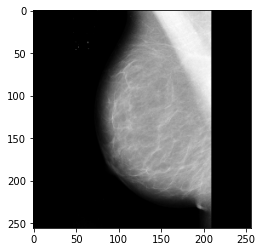
\includegraphics{img/tarea_2_4_1.png}
\caption{RE}
\end{figure}

\begin{Shaded}
\begin{Highlighting}[]
\CommentTok{\# Imagen de ejemplo (Imagen binarizada limpia)}
\NormalTok{plt.imshow(clean\_imgs\_bin[}\DecValTok{13}\NormalTok{], cmap}\OperatorTok{=}\StringTok{\textquotesingle{}gray\textquotesingle{}}\NormalTok{)}
\NormalTok{plt.show()}
\end{Highlighting}
\end{Shaded}

\begin{figure}
\centering
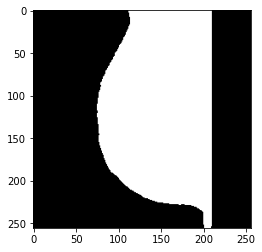
\includegraphics{img/tarea_2_4_2.png}
\caption{RE}
\end{figure}

Finalmente, todas las imágenes limpias se almacenan en el directorio de
la aplicación para que puedan usarse dentro de ella.

\begin{Shaded}
\begin{Highlighting}[]
\CommentTok{\# Almacenar las mamografías limpias en la carpeta de la aplicación}
\NormalTok{app\_dir }\OperatorTok{=} \StringTok{\textquotesingle{}../app/img/\textquotesingle{}}
\CommentTok{\# Obtener los números de imagen en el orden en el que se importaron al entorno}
\NormalTok{find\_nums }\OperatorTok{=}\NormalTok{ re.}\BuiltInTok{compile}\NormalTok{(}\StringTok{\textquotesingle{}\textbackslash{}d}\SpecialCharTok{\{3\}}\StringTok{\textquotesingle{}}\NormalTok{)}
\NormalTok{imgs\_nums }\OperatorTok{=} \BuiltInTok{list}\NormalTok{(}\BuiltInTok{map}\NormalTok{(}\KeywordTok{lambda}\NormalTok{ filename: }\BuiltInTok{int}\NormalTok{(find\_nums.findall(filename)[}\DecValTok{0}\NormalTok{]), imgs\_filenames))}

\ControlFlowTok{for}\NormalTok{ img\_scale, img\_clean, img\_bin, img\_num }\KeywordTok{in} \BuiltInTok{zip}\NormalTok{(imgs\_scale, clean\_imgs, clean\_imgs\_bin, imgs\_nums):}
\NormalTok{    cv.imwrite(app\_dir }\OperatorTok{+} \BuiltInTok{str}\NormalTok{(img\_num) }\OperatorTok{+} \StringTok{\textquotesingle{}\_scale.png\textquotesingle{}}\NormalTok{, img\_scale)}
\NormalTok{    cv.imwrite(app\_dir }\OperatorTok{+} \BuiltInTok{str}\NormalTok{(img\_num) }\OperatorTok{+} \StringTok{\textquotesingle{}\_clean.png\textquotesingle{}}\NormalTok{, img\_clean)}
\NormalTok{    cv.imwrite(app\_dir }\OperatorTok{+} \BuiltInTok{str}\NormalTok{(img\_num) }\OperatorTok{+} \StringTok{\textquotesingle{}\_bin\_clean.png\textquotesingle{}}\NormalTok{, img\_bin)}
\end{Highlighting}
\end{Shaded}

\hypertarget{referencias}{%
\subsection{Referencias}\label{referencias}}

Liu, C.-C., Tsai, C.-Y., Tsui, T.-S., \& Yu, S.-S. (2012). An improved
GVF snake based breast region extrapolation scheme for digital
mammograms. Expert Systems with Applications, 39(4), 4505-4510.
\url{https://doi.org/10.1016/j.eswa.2011.09.136}

Liu, C.-C., Tsai, C.-Y., Liu, J., Yu, C.-Y., \& Yu, S.-S. (2012). A
pectoral muscle segmentation algorithm for digital mammograms using Otsu
thresholding and multiple regression analysis. Computers \& Mathematics
with Applications, 64(5), 1100-1107.
\url{https://doi.org/10.1016/j.camwa.2012.03.028}

OpenCV. (2021, 9 marzo). OpenCV: Morphological Transformations.
\url{https://docs.opencv.org/master/d9/d61/tutorial_py_morphological_ops.html}

\end{document}
